\documentclass[11pt,a4paper]{article}
\usepackage{acl2015}
\usepackage{times}
\usepackage{url}
\usepackage{latexsym}
\usepackage{algorithm} 
\usepackage{algorithmic}
\usepackage{bm}
\usepackage{graphicx}
\usepackage{enumitem}
\usepackage{multirow}
\usepackage{todonotes}
\usepackage{tikz}
\usetikzlibrary{arrows}
\usepackage{caption}
\usepackage{subcaption}
\usepackage{titlesec}
\title{Semantic understanding of natural language text using distant supervision}
\author{Sudha Rao (raosudha@cs.umd.edu)}
\begin{document}
\maketitle
\section{Motivation}
The beauty of natural language lies in the fact that it allows us to express the same thought in very different ways. But this makes it hard for machines to interpret natural languages since machines are good at memorizing data but pretty bad at generalizing from them. For e.g. a human can easily identify that the two sentences ``The boy wants the girl to believe him'' and ``The boy has a desire to be believed by the girl'' mean the same but it is difficult for a machine to do so. What can help machines in this case is if they can work with a kind of representation that abstracts away from various syntactic idiosyncrasies and captures the very meaning of the sentence. Such semantic level of understanding of text is becoming more and more necessary as the field of natural language processing (NLP) tries to solve problems that are closer to natural language understanding. 

Most of these NLP systems learn from examples and therefore need annotated data to train on. However, manually annotating data with semantic information is expensive and time-consuming since it requires a linguistic expert in the loop. The availability of rich knowledge bases in recent times has given rise to an indirect way of gathering training data called distant supervision \cite{mintz2009distant}. To elaborate, suppose we are interested in extracting relations between proteins from a text and we have database that contains information about protein interactions. Then in this technique, for each pair of proteins that appears in the database, we would find all sentences containing the two proteins in a large unlabeled corpus and use them as our training data. 
 
My research work focuses on how we can use such distant supervision techniques for solving problems that require deeper semantic understanding of text. In subsequent sections I will discuss some of my work that fall under this category and also discuss how these ideas are relevant to work at Facebook Research.

\begin{figure}
\centering
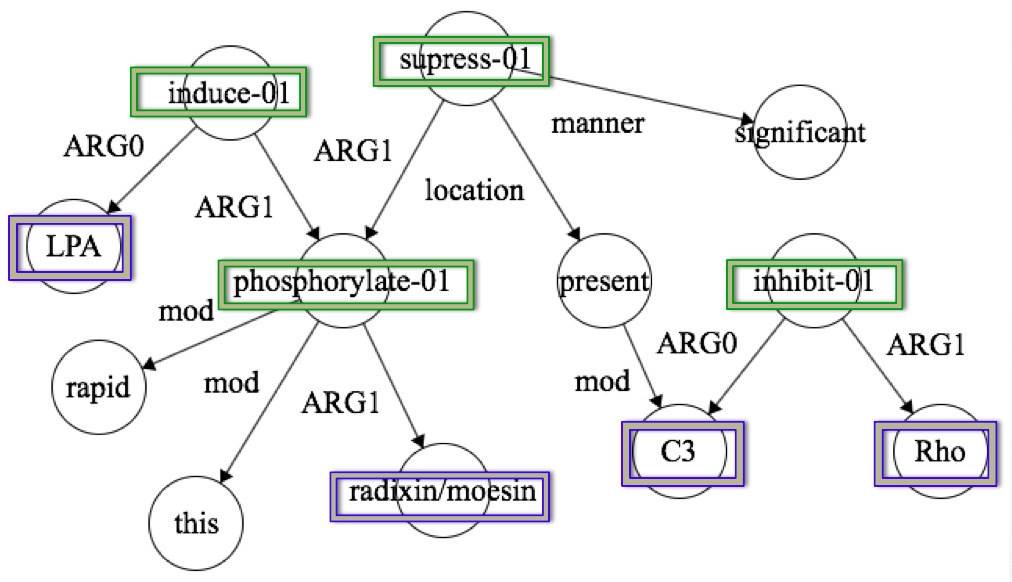
\includegraphics[width = .5\textwidth]{EgAMR}
\caption{AMR for sentence \textit{``This LPA-induced rapid phosphorylation of radixin/moesin was significantly suppressed in the presence of C3 toxin, a potent inhibitor of Rho''}}
\label{amr_eg}
\end{figure}
\section{Relation extraction}
An important aspect of natural language understanding is identifying relationships between different entities in a text. For e.g. consider the following sentence from biomedical literature: \textit{``This LPA-induced rapid phosphorylation of radixin/moesin was significantly suppressed in the presence of C3 toxin, a potent inhibitor of Rho''}. Figure ~\ref{amr_eg} shows its Abstract Meaning Representation (AMR) \cite{banarescu2013abstract} which is a semantic representation that tries to capture the overall meaning of the sentence in the form of a graph structure. Identifying relations between proteins in this sentence becomes much easier for a machine given the AMR, as opposed to when given the original sentence. For e.g. the subtree rooted at induce-01 shows that \textit{LPA induces phosphorylation}, subtree rooted at phosphorylate-01 shows \textit{this phosphorylation occurs on radixin/moesin} and so on. 

During my internship at ISI (Information Science Institute) this summer, I worked with Dr. Daniel Marcu and Dr. Kevin Knight on developing a feedforward neural network model that made use of the AMR path information to extract relations from biomedical text. We trained our model on huge amounts of data that we labelled automatically using distant supervision from a biological knowledge base called BioPax. This model gave us an absolute improvement of 0.52 in recall (with 0.15 increase in F1) over an existing baseline model. This work is under preparation.


\section{Semantic parsing}
For semantic representations like AMR to be useful for NLP tasks, we need methods that can automatically parse sentences into these representations. There has been some work on AMR parsing \cite{flanigan-EtAl:2014:P14-1}, \cite{DBLP:conf/emnlp/PustHKMM15}, etc including ours \cite{rao2015parser}, where we developed a novel technique to parse English sentences into AMR using SEARN \cite{daume2009search}, a learning to search approach to solving structured prediction task. Unlike our predecessors, we modeled the concept (nodes) and the relation (edges) learning in a unified framework and showed an improvement of 2-6\% over the baseline on different datasets. 

Though there has been some promising work on semantic parsing, accuracy of these parsers is much lower than those we can get for syntactic parsers (e.g. dependency parsers) making them less usable. Paucity of annotated data to learn from is one of the main reasons that makes semantic parsing challenging for machines. But humans do not need such huge amounts of data to efficiently parse a sentence for its meaning. This is because they learn to generalize using their common sense/prior knowledge. Following this insight, I plan on building a semantic parser that can be distantly supervised using knowledge bases like the Wikipedia, DBPedia, OpenCyc, Freebase, etc.

\section{Zero pronoun resolution}
I first came to appreciate the usefulness of distant supervision in my work on zero pronoun resolution for Chinese \cite{rao-EtAl:2015:NAACL-HLT} in a dialogue setting. Chinese being a ``pro-drop'' language tends to drop pronouns when they are implicit from the context. The corresponding task of resolving the dropped pronouns to one of the speakers (or to an outside entity in case of third person pronoun) is called zero pronoun resolution. In our work we developed a novel sequential model that explicitly tracked the conversation focus in a dialogue to resolve the zero pronouns. 

To train our model, we needed annotated data and it was expensive to have humans annotate data for us. So we turned to distant supervision. English, unlike Chinese, is not a pro-drop language and mentions pronouns explicitly. Also there is huge amount of readily available Chinese-English parallel corpora. We developed a method to automatically label the zero pronouns in Chinese using the pronouns in its English translation, allowing us to have a large amount of labelled data to train on. This kind of a distant supervision, even though noisy, gave significant improvements over purely supervised approaches.

\section{Applications to Microsoft Research}
I believe that my current expertise in semantics puts me in a good position to contribute to the ongoing research in computational linguistics at Microsoft. The BioNLP project at Microsoft that aims at extracting structured information from biomedical text can make use of deeper semantic representation like AMR. Distant supervision from knowledge bases like the Freebase will enable semantic parsers to generalize beyond seen data and help them parse unseen sentences better. In general, designing models based on semantics will make machine understanding closer to human understanding and thus allow us to build applications that are more natural language friendly. 

\bibliographystyle{acl}
\bibliography{ResearchOverview}

\end{document}


